\documentclass[answers,12pt]{exam}
%\linespread{1.5}
\usepackage{epsfig}
\usepackage{amsmath}
\usepackage{amsfonts}
\usepackage{verbatim}
\usepackage[version=4]{mhchem}
\usepackage{multicol}
\usepackage{enumitem,amssymb}
\newlist{todolist}{itemize}{2}
\setlist[todolist]{label=$\square$}
\usepackage{graphicx}
\usepackage{hyperref}
\usepackage{siunitx}
\usepackage{xspace}
\usepackage{pgfplots}
\hypersetup{
    colorlinks=true,
    linkcolor=blue,
    filecolor=magenta,
    urlcolor=cyan,
}
\pagestyle{empty}


\pagestyle{head}
\runningheadrule
\firstpageheader{\textbf{Math 550 HW0}}{\textbf{}}{\textbf{Name: Hayden Floyd}}
%\runningheader{Math 307}{First Exam}{page \thepage\ of \numpages}

\newcommand{\hor}[1]{\hspace{#1}}
\newcommand{\ver}[1]{\vspace{#1}}
\newcommand{\p}[1]{\left( {#1} \right)}
\newcommand{\abs}[1]{\left| #1 \right|}
\newcommand{\sq}[1]{\left[ #1 \right]}
\newcommand{\bra}[1]{\left< #1 \right>}
\newcommand{\ds}{\displaystyle}
\newcommand{\mysol}[1]{\begin{solution} #1 \end{solution}}

\printanswers
\begin{document} 
	\begin{questions}
		\question Write a matlab code that uses finite differences to compute the first derivative of $$f(x) = \exp(\sin(x))$$ on the interval $0\leq x\leq 2\pi$. Use second-order centered differences on internal grid points and first-order one-sided differences at endpoints.
        \begin{parts}
			\part Show a graph of the exact analytic solution $f'(x)$ and your numerical solution $f'_n(x)$.
            \mysol{\\\\
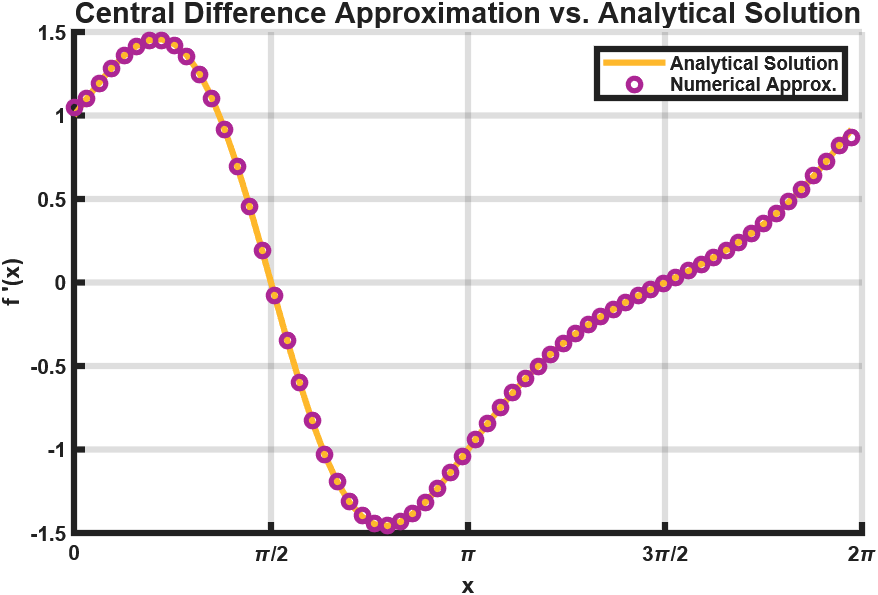
\includegraphics[width=1\linewidth]{math550hw0plot1(2).png}
            
            }
			
			\part Show a relative error convergence plot by plotting the relative error on the y-axis and the grid size N on the x-axis. Measure relative error as $$Err=\frac{||f'(x)-f'_n(x)||_p}{||f'(x)||_p}.$$ Plot the error using both the $p=\infty$, 2 norms in a log-log scale. The relative errors should be lines with slopes $1$ and $3/2$ respectively, i.e. it scales with $\frac{1}{N}$, $\frac{1}{N^{3/2}}$. Extra Credit: The $3/2$ slope is strange, why is that happening?
            \mysol{\\As a general note, I was unsure of what this problem was asking me to plot. It sounds like I needed two lines with different slopes and a smoother line.\\
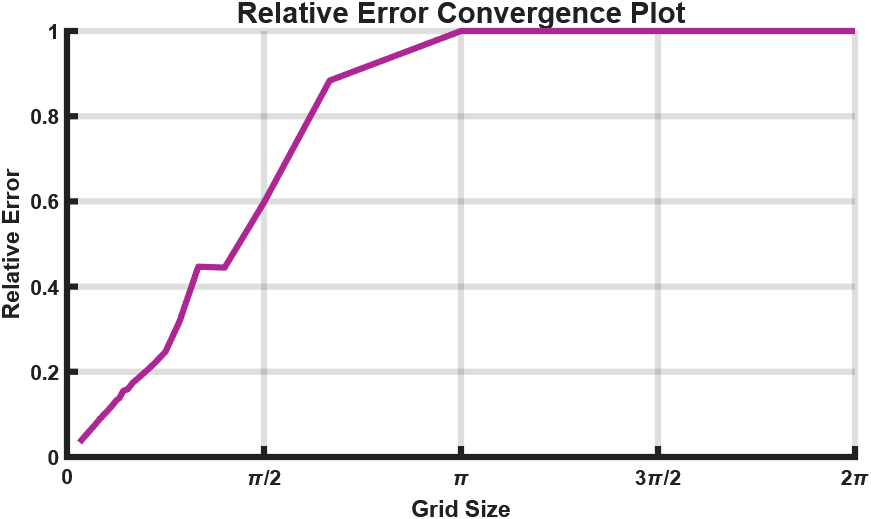
\includegraphics[width=1\linewidth]{math550hw0plot3.png}
            
            }
\end{parts}	

\question Repeat problem 1 but compute the second derivative $f''(x)$. Assume periodicity and wrap around the grid instead of using one-sided finite differences.
\mysol{\\\\
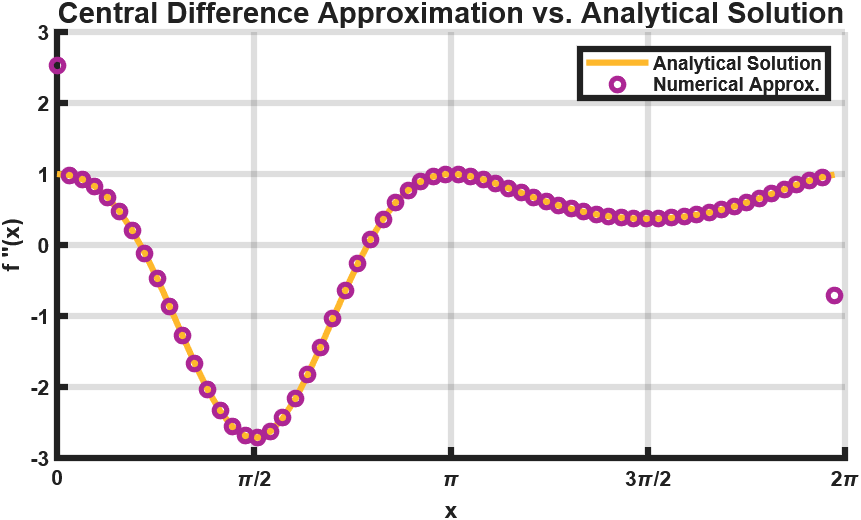
\includegraphics[width=1\linewidth]{math550hw0plot2.png}\\ As a note, I checked my endpoints many times and am unsure if they are correct or not.\\
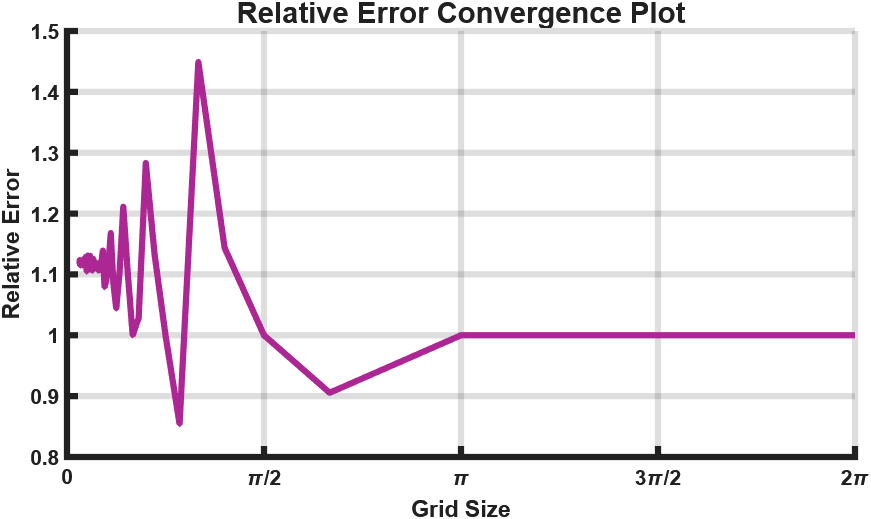
\includegraphics[width=1\linewidth]{math550hw0plot4.png}\\
Again, I am unsure of what the error convergence plot is supposed to be. I do have my code files included in my github repo, and hoping I can work to improve my work and resubmit.

}


\question Consider the ODE $$\frac{d^2u}{dx^2} + \sin{(x)} \frac{du}{dx} + u(x) = f(x)$$ defined on $0\leq x\leq 5$. Solve the ODE using second-order finite difference methods with the Dirichlet conditions. Use $u(x)=\sin (x)$ to test your solution by finding boundary conditions and the necessary forcing function $f(x)$. Show an error plot that proves your method converges with second order.

    \mysol{\\ This is not an error convergence plot, but I was unable to implement this correctly in Matlab in time. Here is a plot of the absolute error for our ODE where the spacing $h=1$ on $0\leq x\leq 5$.
    \\
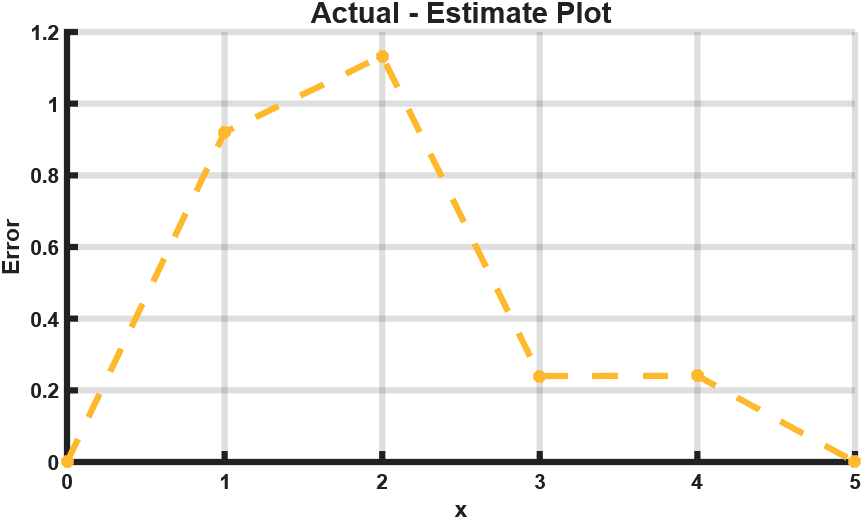
\includegraphics[width=1\linewidth]{math550hw0plot5.png}\\

    }


\question Use finite difference methods to solve the Poisson equation $\nabla^2u=f(x,y)$ in the domain $x\in[0, 5], y\in[0,5]$. Use the test solution $u(x,y)=\sin(x)\cos(y)$.

\begin{parts}
	\part Apply Dirichlet conditions on all boundaries so that $u(x,y)$ satisfies the PDE and the boundary conditions, and show a plot of your solution and a second order convergence plot (similar to the first three problems).
    \mysol{
I don't know where to start coding with this one, so I'm just going to conceptually explain what I understand with this problem. We have our boundaries, so we can choose $i$ to be our x-axis on our grid and $j$ to be our y-axis, with positive values being right and up respectively. To discretize our finite difference method, we let our function $f_{i,j}=\frac{U_{i,j+1}-2U_{i,j}+U_{i,j-1}}{\Delta x^2} + \frac{U_{i+1,j}-2U_{i,j}+U_{i-1,j}}{\Delta y^2}$. To code, we choose $i$ or $j$ to be the inner loop ("fast index") and the other to be the outer loop ("slow index"). We calculate each $U_{i,j}$ and use the $U$ matrix to solve for the vector of unknowns.
    }
	
	\part Modify your code to apply Neumann conditions on all boundaries. This won't work. Why not? - both in terms of the linear algebra and in terms of the actual PDE we want to solve. Suggest a solution to the issue.
    \mysol{
    The Neumann conditions are when we know the derivative's boundaries. Applying them without modifying the rest of our code would not work, because the Neumann conditions has a different matrix and rhs vector format.
    }
	
\end{parts}


	\end{questions}

\end{document}